%%%%%%%%%%%%%%%%%%%%%%%%%%%%%%%%%%%%%%%%%%%%%%%%%%%%%%%%%%%%%%%%%%%%%%%%
%Desarrollo de un juego para Nintendo DS | Trabajo de Fin de Grado
% Escuela Politécnica Superior de la Universidad de Alicante
% Realizado por: Carla Maciá Díez
% Contacto: carlamd1997@hotmail.com / cmd23@alu.ua.es
%%%%%%%%%%%%%%%%%%%%%%%%%%%%%%%%%%%%%%%%%%%%%%%%%%%%%%%%%%%%%%%%%%%%%%%%


\chapter{Nintendo DS} 

La \textbf{Nintendo DS} es una videoconsola portátil de la compañía de origen japonés; \textbf{Nintendo}. Creada para suceder a la Game Boy Advance, se lanzó al mercado el \textbf{21 de noviembre de 2004 en Estados Unidos}, retrasándose su fecha de lanzamiento en \textbf{Japón al 2 de diciembre} y en\textbf{ Europa al 5 de marzo del año siguiente} con un \textbf{precio de 149.99€}. La consola original y sus versiones posteriores alcanzaron un total de \textbf{154,90 millones unidades vendidas} en todo el mundo y su videojuego más vendido fue el \textbf{New Super Mario Bros}, con un total de 30,80 millones de copias vendidas.

\vspace{0.5cm}

\begin{figure}[htbp]
\centering
  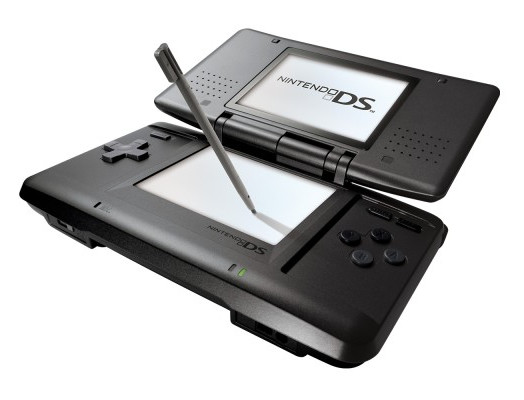
\includegraphics[width=0.4\textwidth]{archivos/nds.jpg}
  \caption{Nintendo DS}
  \textbf{Fuente:} \href{https://www.nintendo.co.uk/Nintendo-DS/Nintendo-DS-Family-Nintendo-UK-s-official-site-Nintendo-DS-Nintendo-DSi-Nintendo-DSi-XL-116380.html}{Nintendo}
  \label{fig:nds1}
\end{figure}

\vspace{0.5cm}

La consola consta de \textbf{ dos pantallas LCD} retroiluminadas con brillo ajustable, siendo una de ellas (la inferior) \textbf{ táctil}, un  \textbf{pad de direcciones},  \textbf{seis botones de acción} (A,B,X,Y, R y L) , \textbf{dos botones de control} (Start y Select) y un \textbf{micrófono}. En su interior posee \textbf{dos procesadores}, un \textbf{ARM946E-S} de 67 MHz que, en general, se encarga de la mayor parte del trabajo ejecutando los \textbf{juegos de NDS} y un \textbf{ARM7TDMI} de 33 MHz, que mueve los juegos de \textbf{GBA} y algunas funciones Wi-Fi. Profundizaremos en ambos procesadores más adelante.

\vspace{0.5cm}

Como curiosidad, las siglas DS significan \textbf{Developer's System} (Sistema de desarrolladores) ya que según la compañía, este sistema ofrece muchas herramientas para que los desarrolladores puedan innovar en sus creaciones. No obstante, también hicieron oficial que estas siglas también hacían referencia a \textbf{Dual Screen}, por su doble pantalla.

\vspace{1cm}

\section{Versiones}

Ahora que conocemos un poco más la Nintendo DS original, es importante que analicemos sus posteriores ediciones ya que nuestro juego debe funcionar en cualquiera de ellas. Debemos conocer qué diferencias significativas existen y tenerlas en cuenta a la hora de desarrollar el juego. Así pues vamos a ir revisando la familia de consolas de Nintendo DS y conociendo sus principales cambios.

\vspace{1cm}

%\subsection{Nintendo DS}

%\begin{figure}[htbp]
%\centering
  %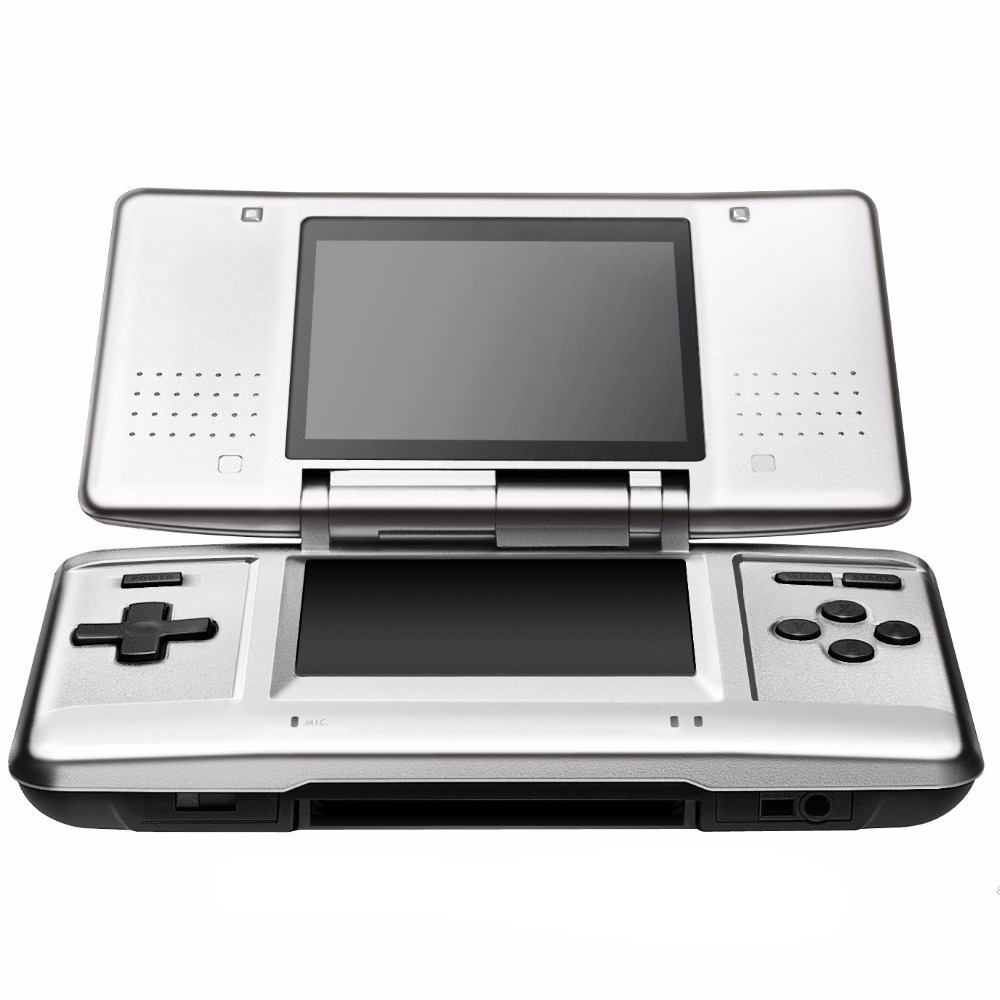
\includegraphics[width=0.3\textwidth]{archivos/nds2.jpg}
 % \caption{Nintendo DS}
  %\label{fig:nds2} %si cambio esto se irá la ref a la *??
%\end{figure}

\subsection{Nintendo DS Lite}

Fue creada en \textbf{2006} por Nintendo, es ligeramente \textbf{más pequeña} que su predecesora e incluía una \textbf{carcasa} más elegante. Algunos \textbf{botones} fueron \textbf{relocalizados} y añadía la función de poder elegir entre \textbf{4 niveles de brillo} a diferencia de la original, que solo podía ajustarse al mínimo o al máximo.

\vspace{0.5cm}

\begin{figure}[htbp]
\centering
  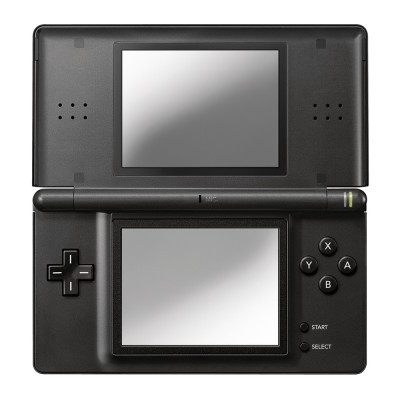
\includegraphics[width=0.3\textwidth]{archivos/ndslite.jpg}
  \caption{Nintendo DS Lite}
    \textbf{Fuente:} \href{https://www.nintendo.co.uk/Nintendo-DS/Nintendo-DS-Family-Nintendo-UK-s-official-site-Nintendo-DS-Nintendo-DSi-Nintendo-DSi-XL-116380.html}{Nintendo}
  \label{fig:ndslite}
\end{figure}

\vspace{1cm}

\subsection{Nintendo DSi}

Salió a la venta a finales de \textbf{2008 en Japón} y en \textbf{2009 en el restro del mundo} y se trata de una \textbf{revisión} del modelo de la Nintendo DS Lite. Si bien mantiene muchas características intactas, hay algunas otras que se deben destacar.

\vspace{0.5cm}

\begin{figure}[htbp]
\centering
  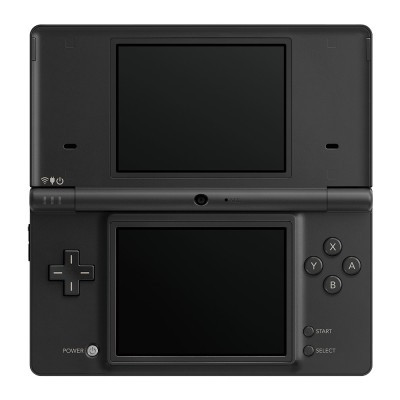
\includegraphics[width=0.3\textwidth]{archivos/ndsi.jpg}
  \caption{Nintendo DSi}
    \textbf{Fuente:} \href{https://www.nintendo.co.uk/Nintendo-DS/Nintendo-DS-Family-Nintendo-UK-s-official-site-Nintendo-DS-Nintendo-DSi-Nintendo-DSi-XL-116380.html}{Nintendo}
  \label{fig:ndsi}
\end{figure}

\vspace{0.5cm}

El primer cambio notable y que a mucha gente no le agradó fue que \textbf{dejaba de ser compatible} con los juegos de \textbf{GBA}, pues ya no poseía ranura para los cartuchos. Introdujeron una \textbf{cámara delantera} y otra \textbf{trasera}, ambas de 0.3 megapíxeles, con las que podías hacer fotos y editarlas mediante un programa llamado \textbf{Cámara DSi} que venía instalado en la consola por defecto.  Poseía también una ranura para \textbf{tarjetas SD}, en las que podías guardar las fotos de la cámara así como los programas o juegos que descargases de la \textbf{Tienda Nintendo DSi}.

\vspace{0.5cm}

Por último, otras mejoras o diferencias frente a sus modelos originales son una \textbf{mejora de la calidad del audio}, \textbf{aumento} de la \textbf{memoria interna y RAM}, el procesador principal \textbf{ARM9} pasó a ser de 133 MHz (\textbf{aumentando su velocidad}), un \textbf{aumento} ligero del \textbf{tamaño de las pantallas} y \textbf{reducción} de la \textbf{duración de la batería} a 16 horas, siendo de 18 horas y media las originales.

\vspace{0.5cm}

El \textbf{menú principal} de la consola es completamente distinto al de la DS original, pasando a ser bastante \textbf{más personalizable} y con una gran variedad de programas, los cuales algunos de ellos se mantenían desde la DS como el \textbf{Picto-Chat} o la \textbf{Descarga DS}.

\vspace{0.5cm}

\begin{figure}[htbp]
\centering
  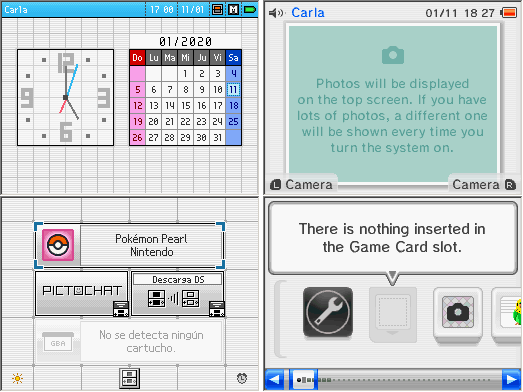
\includegraphics[width=0.6\textwidth]{archivos/nds-ndsi-menu.png}
  \caption{Menú de Nintendo DS (izquierda) frente al de Nintendo DSi (derecha)}
  \label{fig:menu-comparacion} %si cambio esto se irá la ref a la *??
\end{figure}

\vspace{0.5cm}

Fué la primera consola portátil en tener \textbf{bloqueo regional}, no permitiendo que juegos desarrollados en países extranjeros se ejecutasen en la consola si esta era originaria del mismo país.

\vspace{1cm}

\subsection{Nintendo DSi XL}

Se trata de un modelo adicional de NDSi que salió a la venta en \textbf{Japón en 2009}, donde originalmente se bautizó como Nintendo DSi LL, llegando a \textbf{España en 2010} donde pasó a llamarse Nintendo DSi XL.

\vspace{0.5cm}

\begin{figure}[htbp]
\centering
  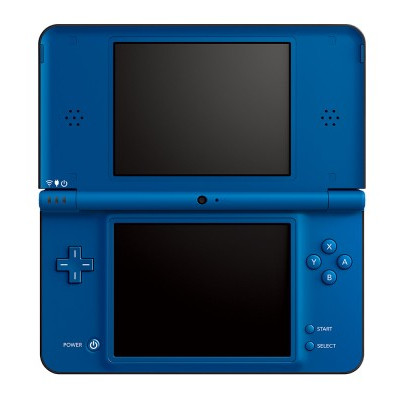
\includegraphics[width=0.3\textwidth]{archivos/ndsixl.jpg}
  \caption{Nintendo DSi XL}
    \textbf{Fuente:} \href{https://www.nintendo.co.uk/Nintendo-DS/Nintendo-DS-Family-Nintendo-UK-s-official-site-Nintendo-DS-Nintendo-DSi-Nintendo-DSi-XL-116380.html}{Nintendo}
  \label{fig:ndsixl} %si cambio esto se irá la ref a la *??
\end{figure}

\vspace{0.5cm}

El principal cambio destacable es el considerable aumento del tamaño de la consola como consecuencia del \textbf{aumento del tamaño de las pantallas} (estas tienen aproximadamente \textbf{una pulgada más} comparadas con la NDSi). En general es una consola perfecta para aquellos que tengan alguna discapacidad visual o les sea difícil o incómodo jugar con las anteriores por su tamaño.

\vspace{1cm}

\section{Especificaciones}

En esta sección vamos a conocer los detalles técnicos de la consola y profundizar en los más interesantes para poder entender qué la compone. Podemos ver a continuación una tabla a modo de resumen.

\vspace{0.5cm}

\begin{table}[htbp]

\centering

\begin{tabular}{|l|l|lll}

\cline{1-2}

\textbf{CPU}                & \begin{tabular}[c]{@{}l@{}}ARM946E-S 32bit RISC CPU\\ ARM7TDMI 32bit RISC CPU\end{tabular} &  &  &  \\ \cline{1-2}

\textbf{Velocidad de reloj} & \begin{tabular}[c]{@{}l@{}}(ARM9) 66MHz\\ (ARM7) 33MHz (16MHz en modo GBA)\end{tabular}    &  &  &  \\ \cline{1-2}

\textbf{RAM}                & 4096KB                                                                                     &  &  &  \\ \cline{1-2}

\textbf{VRAM}               & 656KB                                                                                      &  &  &  \\ \cline{1-2}

\textbf{Pantalla}           & 2 pantallas LCD (256x192 px, 3"). Una de ellas táctil.                                                           &  &  &  \\ \cline{1-2}

\textbf{Paleta de colores}  & 18-bit (262144 colores)                                                                    &  &  &  \\ \cline{1-2}

\textbf{Sonido}             & 16 canales de sonido estéreo                                                               &  &  &  \\ \cline{1-2}

\textbf{Comunicación}       & Wifi IEEE 802.11b                                                                          &  &  &  \\ \cline{1-2}

\textbf{Alimentación}       & Batería recargable de ion de litio 850mAh                                                  &  &  &  \\ \cline{1-2}

\textbf{Peso}               & 275g                                                                                       &  &  &  \\ \cline{1-2}

\textbf{Dimensiones}        & 148.7mm × 84.7mm × 28.9mm                                                                  &  &  &  \\ \cline{1-2}

\end{tabular}
\caption{Especificaciones técnicas de la NDS}
\end{table}

Para profundizar más acerca de los procesadores de la consola, su memoria de vídeo, zonas hardware específicas para gráficos, sonido y ROM, visita el \hyperref[anexo]{\textbf{Anexo I}}.

\vspace{1cm}
